\documentclass[fleqn,10pt]{physiome}
% Use option lineno for line numbers 

\articletype{Original}
%% Choose from Original, Retrospective, Review, Letter

\title{Bond Graph Model of Cerebral Circulation: Toward Clinically Feasible Systemic Blood Flow Simulations}
\author[1]{Shan Su}
\author[2]{Pablo J. Blanco}
\author[3]{Lucas O. M\"{u}ller}
\author[1]{Peter J. Hunter}
\author[1][soroush.safaei @auckland.ac.nz]{Soroush Safaei}
\affil[1]{Auckland Bioengineering Institute, University of Auckland, New Zealand}
\affil[2]{National Laboratory for Scientific Computing, Petrópolis, Brazil}
\affil[3]{Department of Mathematics, University of Trento, Italy}


%% The following lines can be omitted when submitting;
%% information will be added by editors
\publicationdate{25 August 2020}
\editor{Karin Lundeng\r{a}rd}
\curator{Anand K. Rampadarath}
\submitteddate{25 August 2020}
\accepteddate{25 August 2020}
\citethisas{Su et al. (2020)\\Bond Graph Model of Cerebral Circulation: Toward Clinically Feasible Systemic Blood Flow Simulations. Physiome.}{10.36903/physiome.12859424}

\begin{document}

\maketitle

\begin{abstract}
The primary paper \citet{safaei2018} proposed an anatomically detailed model of the human cerebral circulation that runs faster than real-time on a desktop computer and is designed for use in clinical settings when the speed of response is important. Based on a one-dimensional formulation of the flow of an incompressible fluid in distensible vessels, a lumped parameter model was developed for 218 arterial segments. The proposed model improved simulation speed by approximately 200-fold while preserved accuracy. Bond graph formulation was used to ensure mass and energy conservation. The model predicted the pressure and flow signatures in the body.
\end{abstract}

\keywords{Circulation model, bond graph, 0D model, CellML, OpenCOR}

\primarypubs[10.36903/physiome.12859424]{bibliography}{safaei2018p}

\section{Introduction}
The primary paper \citet{safaei2018} aimed to achieve two goals in cardiovascular system modelling: making the model subject-specific and fast enough to be useful in a clinical setting. An existing cardiovascular model, Anatomically Detailed Arterial Network (ADAN) model \citet{blanco2015}, utilises a detailed geometry of the cardiovascular system and simulates the blood flow by solving 1D version of the Navier-Stokes equations in compliant domains. The primary paper developed a 0D compartmentalised model to predict the haemodynamics of the same subject. The model is formulated as a system of Ordinary Differential Equations (ODE) which is 200x faster to solve, thus enabling real-time simulations. Compared to the 1D model, the 0D model achieved a prediction accuracy of within $5$\%, for the blood flow and pressure during one cardiac cycle. A closed-loop is formed by providing components representing the venous return to the heart. With 218 arterial segments in the body, the model predicted the detailed blood flow signature towards various tissue beds. The model is publicly accessible at Physiome Model Repository: \url{https://models.physiomeproject.org/workspace/5e0}.

\section{Model Description}

In the 0D model, instead of treating blood vessels as a continuum, they were modelled as segments in a compartmentalised manner. A bond graph approach was used to represent each segment of a vessel. Bond graph formulation concerns the mass and energy flows in and out of the vessel, following the fundamental laws of mass and energy conservation. The bond graph components for a blood vessel model include resistance, capacitance, and inductance. Resistance is associated with energy dissipation, while capacitance and inductance are associated with energy storage. The parameters describe the integrated properties of the segment, following the assumptions that blood is an incompressible Newtonian fluid flowing through distensible vessels. 

The resistance of the vessel segments was evaluated from the 1D Navier-Stokes equation, assuming a parabolic flow profile under laminar and stationary flow conditions. The capacitance was evaluated for a homogeneous linear elastic material with constant Young's Modulus, and using the theory of thin shells. The inductance was calculated based on the mass inertial effects. The vessel segments were assumed to have a uniform circular cross-section throughout.

\begin{figure}[ht]
\centering
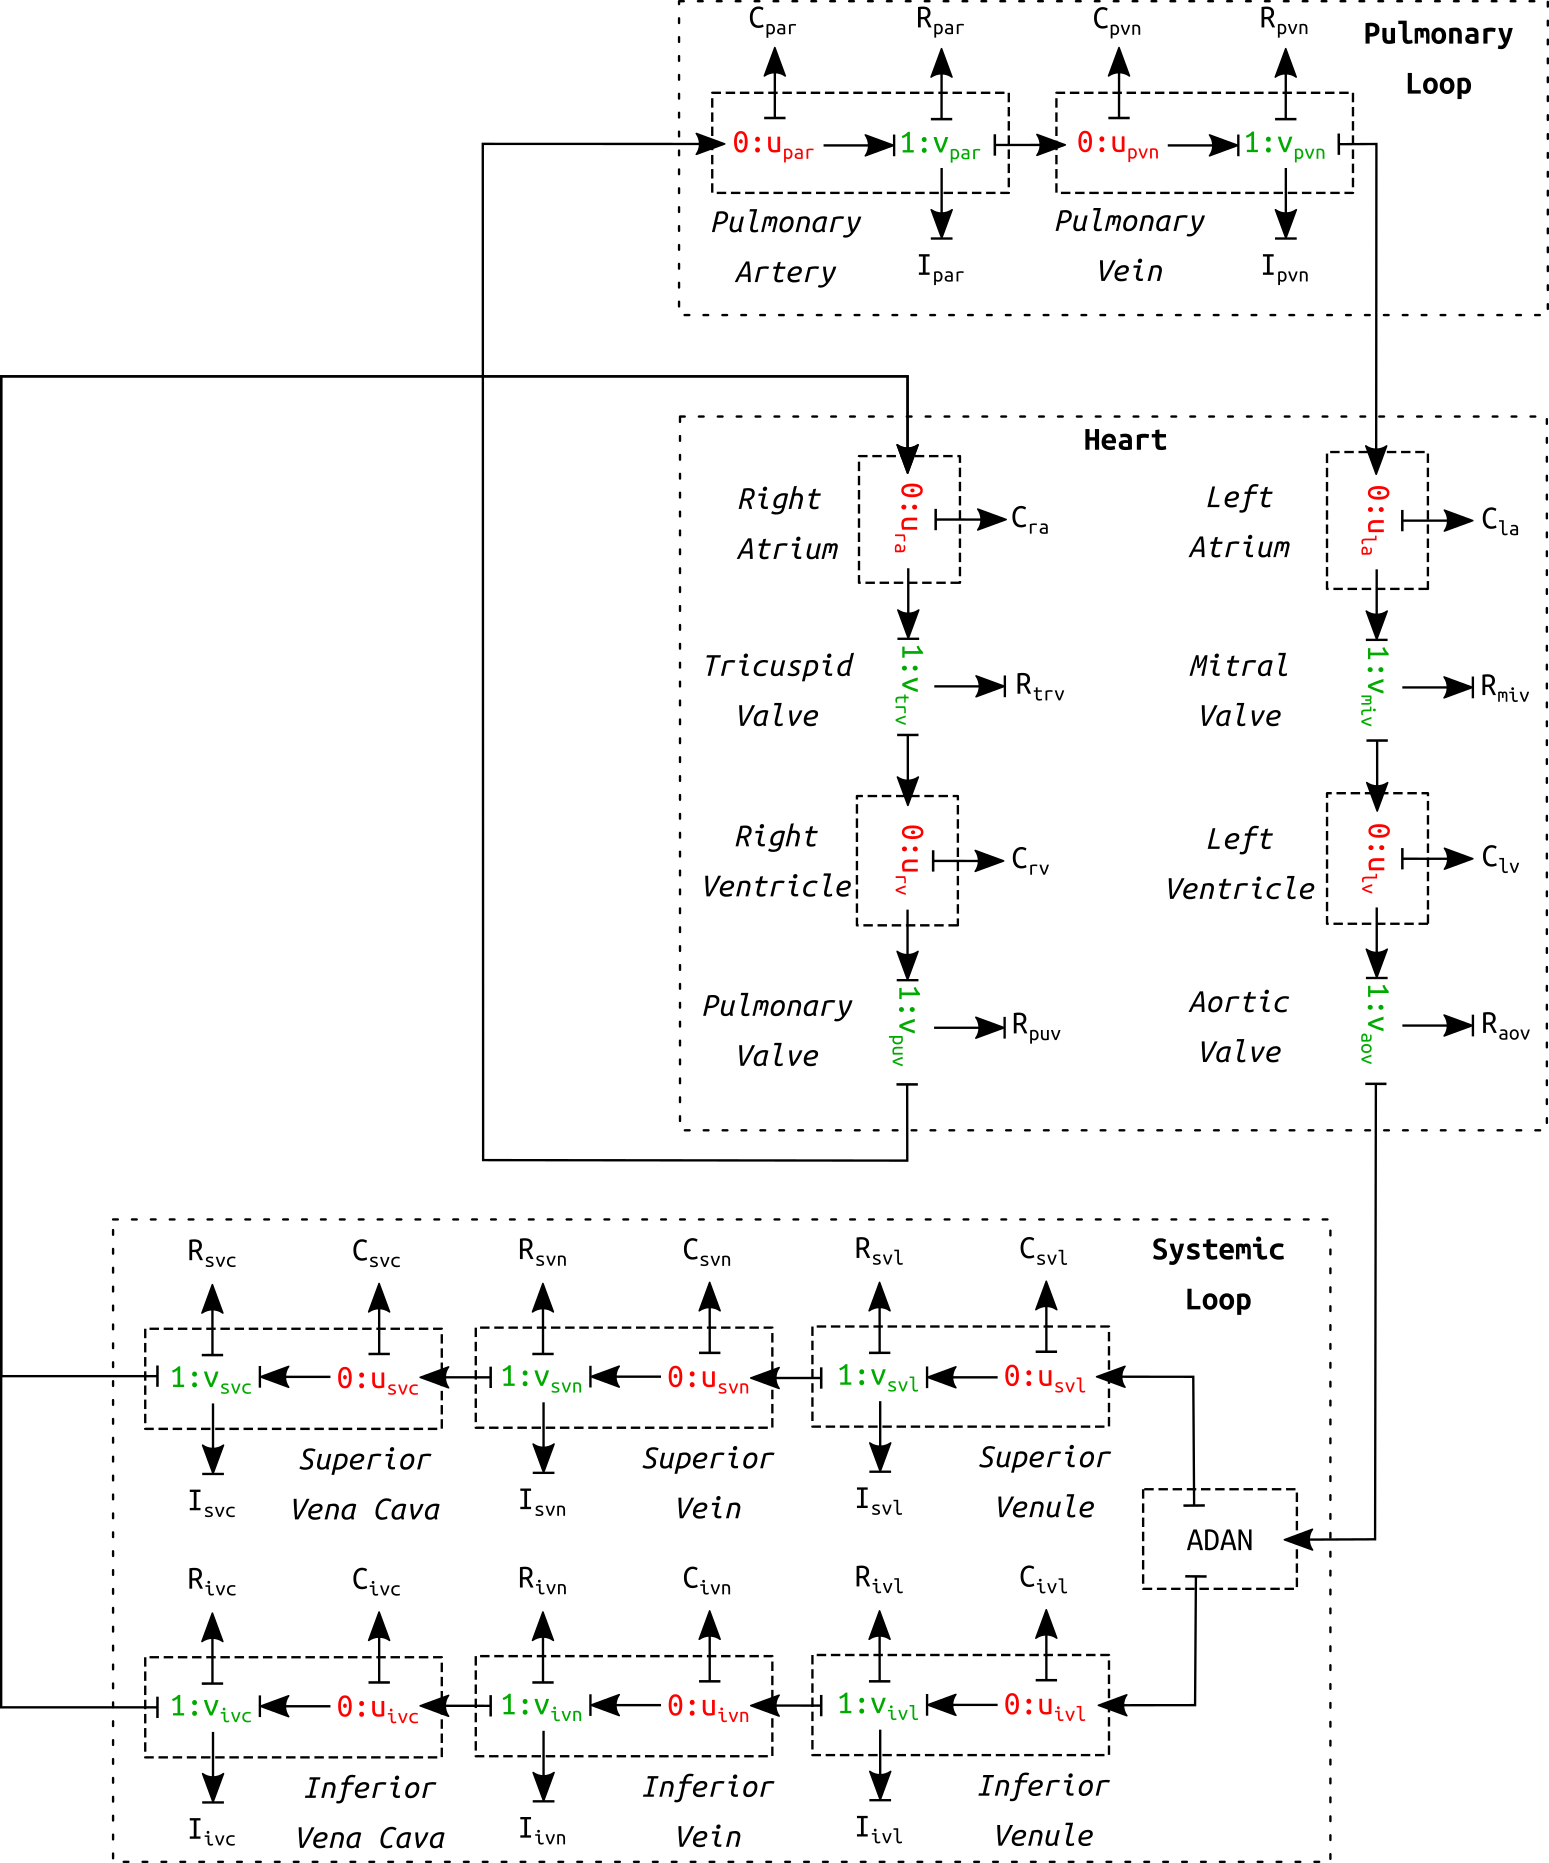
\includegraphics[width=0.85\linewidth]{img/schematics.png}
\caption{Schematic diagram of the circulation model. This is a correction of figure 10 in the primary paper. The circulation model contains six venous vessel segments in the systemic loop as opposed to only one.}
\label{fig:Schematics}
\end{figure}

The complete cardiovascular system model consisted of three parts: heart, systemic loop, and pulmonary loop (see \autoref{fig:Schematics}). The pulmonary circulation was based on the model in \citet{blanco2013}. The heart was modelled as a four-chamber pump, as described in \citet{safaei2018}. The systemic loop covered the rest of the vessels. The arterial geometry was based on ADAN model \citet{blanco2015}. The peripheral blood flow resistance for distal vessels at the end of truncated arteries was evaluated based on \citet{blanco2014}. Six venous components were modelled in the systemic loop. It shall be noted that the schematic in the primary paper (figure 10) mistakenly included only one venous component. \autoref{fig:Schematics} is a corrected version of the schematic of the cardiovascular model. 

By connecting the arterial network and the components in the schematic (see \autoref{fig:Schematics}), a closed-loop was formed to simulate the full cycle of blood flow through the cardiovascular system. A system of ODEs can be formulated that governs the dynamics of the cardiovascular system. 

The model was implemented in CellML. The CellML scripts were arranged as shown in \autoref{fig:CodeArrangement}. The model involves four scripts: BG\_Modules.cellml contains a library of bond graph components, Parameters.cellml collects all the model constants and parameters, Units.cellml stores the unit settings and Main.cellml constructs the final model by mapping the bond graph components following the anatomy.

\begin{figure}[ht]
\centering
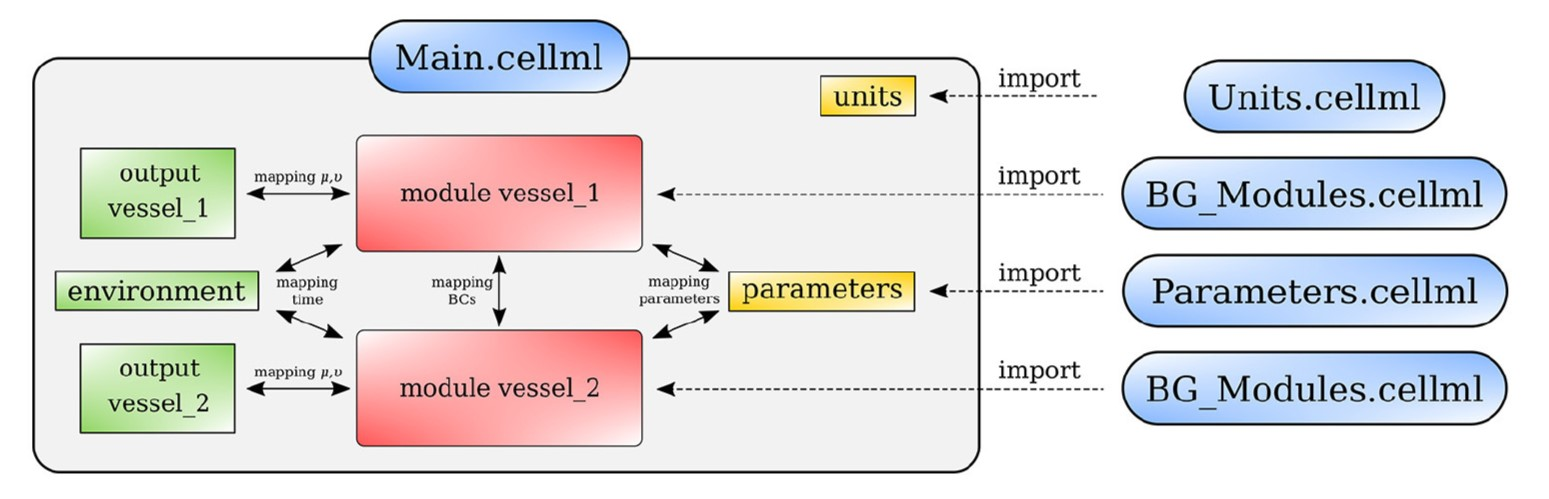
\includegraphics[width=0.9\linewidth]{img/arrangement.jpg}
\caption{Arrangement of the cardiovascular model showing the CellML scripts involved. Main.cellml imports components from the other scripts and constructs the systemic model through mapping of variables between components. For the closed loop model including the cerebral circulation, the main script is named as main\_ADAN-218.cellml.}
\label{fig:CodeArrangement}
\end{figure}

\section{Computational Simulation} 

The simulation file main\_ADAN-218.sedml contains the computational setting for running the model. Open the .sedml file in OpenCOR and click Run Simulation. The simulation requires $10$ cardiac cycles to reach a stabilised periodic solution. The final solution corresponds to the results plotted in figure 15 in the primary paper. The model was run for ten cardiac cycles ($T = 1~\mathrm{s}$) using a $0.001$ s time step, with tolerance $10^{-7}$ and CVODE solver. The computation took about $23~\mathrm{s}$ in a desktop computer with an Intel CORE i5 CPU. To obtain the plots of simulation results, export the csv file from OpenCOR and run MATLAB script csvPlotsGenerator.m (can be found in Physiome Model Repository) to generate the plots.

\section{Model Results}
The simulated results for blood pressure and flow rate for the closed-loop cardiovascular system are reproduced, as shown in \autoref{fig:results}. The results correspond to figure 15 in the primary paper.

\begin{figure}[ht!]
    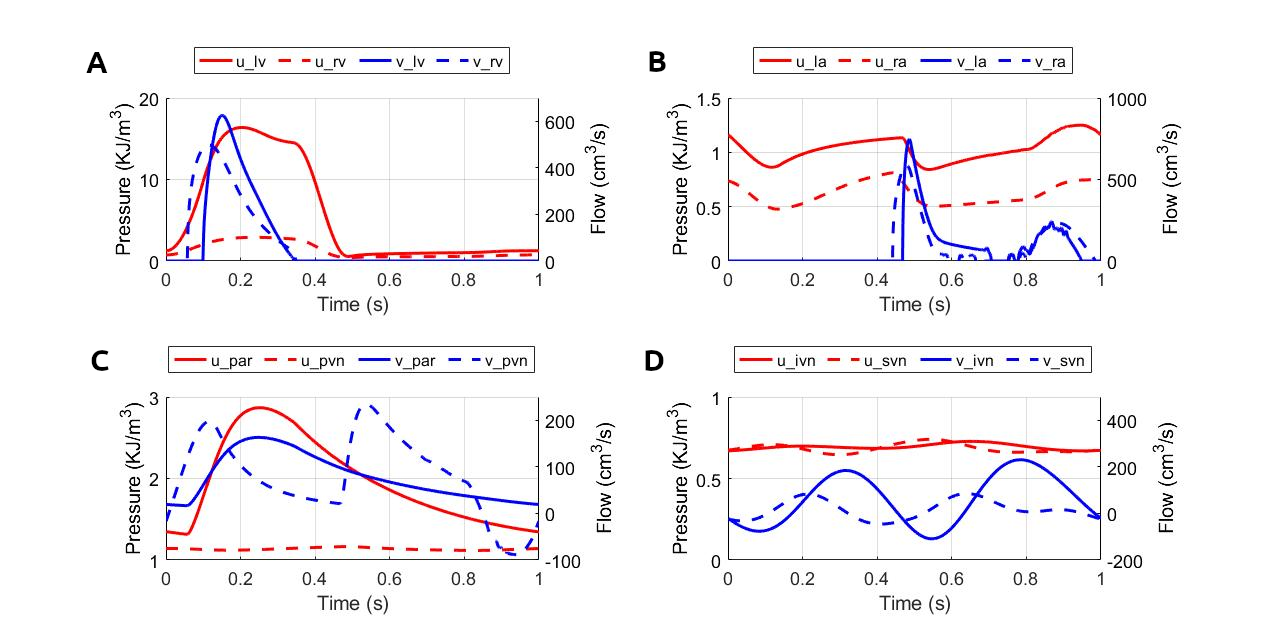
\includegraphics[scale=1.45]{img/figure1.png}
    \includegraphics[scale=1.45]{img/figure2.png}
    \caption{Pressure and flow rate in the main segments during one cardiac cycle. This figure corresponds to figure 15 in the primary paper. u, pressure; v, flow; \textbf{(A)} lv, left ventricle; rv, right ventricle; \textbf{(B)} la, left atrium; ra, right atrium; \textbf{(C)} par, pulmonary arteries; pvn, pulmonary veins; \textbf{(D)} ivn, inferior vena-cava; svn, superior vena-cava; \textbf{(E,F)} ext, external; \textbf{(G,H)} com, common; post, posterior; \textbf{(I,J)} ant, anterior; mid, middle.}
    \label{fig:results}
\end{figure}

\section{Discussion}

The strength of the model is in the near real-time simulation speed compared to 1D solvers, which shows potential in clinical use. The simulated results are sufficiently close to that of the ADAN model, which demonstrates the model reliability. A potential improvement of the model includes developing a model for tapering vessels as many arteries do not satisfy the assumption of uniform radius along the segment. 

\section{Acknowledgements}

SS acknowledges the financial support provided by the Aotearoa Foundation.

\bibliography{bibliography}

\end{document}